\documentclass[12pt]{article}


% imports %
\usepackage[utf8]{inputenc}
\usepackage{biblatex}
\usepackage{graphicx}
\usepackage{hyperref}
\usepackage{subfiles}
\usepackage[italian]{babel}
\usepackage{xcolor,listings}
\usepackage{textcomp}
\usepackage{color}
\usepackage{csquotes}
\usepackage{fancyvrb}
\usepackage{lipsum}

\usepackage[a4paper,bindingoffset=0.2in,%
            left=1in,right=1in,top=1in,bottom=1in,%
            footskip=.25in]{geometry}
% end imports %

\addbibresource{references.bib}


% sql query styke %
\definecolor{codegreen}{rgb}{0,0.6,0}
\definecolor{codepurple}{HTML}{C42043}
\definecolor{backcolour}{HTML}{F2F2F2}
\definecolor{bookColor}{cmyk}{0,0,0,0.90}  

\lstset{upquote=true}

\lstdefinestyle{sql_style}{
    backgroundcolor=\color{backcolour},   
    commentstyle=\color{codegreen},
    keywordstyle=\color{codepurple},
    numberstyle=\numberstyle,
    stringstyle=\color{codepurple},
    basicstyle=\footnotesize\ttfamily,
    breakatwhitespace=false,
    breaklines=true,
    captionpos=b,
    keepspaces=true,
    numbers=left,
    numbersep=10pt,
    showspaces=false,
    showstringspaces=false,
    showtabs=false,
}
\lstset{style=sql_style}

\newcommand\numberstyle[1]{%
    \footnotesize
    \ttfamily
    \ifnum#1<10 0\fi#1 |%
}

% commands %
\renewcommand{\contentsname}{Contenuti}

% end commands%


\begin{document}
\begin{titlepage}
    \begin{center}
        \vspace*{1cm}

        \Huge
        Elaborato dell'esame di Stato \\ su \\ 'Tourm - Gestione audioguide'

        \vspace{1.5cm}

        \begin{center}
            
\includegraphics[scale=0.08]{images/repubblica.png}
        \end{center}

        \normalsize
        Studente: Riccardo Calligaro, classe 5IA\\
        Relatori: Daniele Cappellazzo, Giancarlo Ronchi\\
        Tutor: Donatella Panciera

        \vfill

        ITIS C. Zuccante\
        A. S. 2020/2021

    \end{center}
\end{titlepage}
\newgeometry{left=0.787402in,right=0.787402in,top=1in,bottom=1in}



\newpage

% start of document %
\newpage

\thispagestyle{plain}
\begin{center}
    \vfill
    \Huge
    \textbf{Abstract}
    \vspace{2cm}

\end{center}
\subfile{sections/abstract}
\vfill


% table of contents %
\newpage
\tableofcontents
\newpage
% end table of contents %

\section{Introduzione}
\subsection{Il progetto}
\begin{center}
    \begin{figure}[htp]
        \centering
        
\includegraphics[width=7cm]{images/tourm_logo_transparent.png}
        \vspace{-2.7\baselineskip}
    \end{figure}
\end{center}

\textbf{Tourm} si propone di raggiungere i seguenti obiettivi:
\begin{itemize}
	\item sviluppare una \textbf{applicazione per smartphone}, disponibile sia su ambiente iOS che Android, destinata all’utente finale per consentirgli di:
	\begin{itemize}
	    \item scaricare l'applicazione attraverso un codice QR presente all'interno della villa
		\item accedere alla parte espositiva dell'applicazione con il codice del biglietto acquistato online o allo sportello di vendita.
		\item interagire con le esposizioni automatizzando la riproduzione di spiegazioni audio pre-registrate
		\item interagire con le esposizioni scannerizzando un codice QR che permette di leggere un articolo e ascoltare l'audioguida associata
		\item ricevere notifiche automatiche sulla disponibilità di visite guidate o eventi
	\end{itemize}
    \item sviluppare una \textbf{portale web amministrativo} destinato agli organizzatori per consentirgli di:
	\begin{itemize}
	    \item accedere al conteggio effettivo dei visitatori
		\item visualizzare statistiche riguardo le esposizioni e le interazioni fatte dagli utenti 
		\item chiudere o aprire l’accesso alle stanze
	\end{itemize}
    \item sviluppare un'\textbf{infrastruttura di rete} sicura, veloce e affidabile che permette ai visitatori di:
    \begin{itemize}
        \item collegarsi a una rete wireless gratuita senza accesso ad internet
        \item utilizzare l'applicazione senza nessun costo di dati mobili
        \item utilizzare la rete in modo sicuro senza doversi preoccupare di eventuali minacce
    \end{itemize}
    e ai gestori di: 
    \begin{itemize}
        \item utilizzare dei dispositivi specifici per accedere al pannello di amministrazione
    \end{itemize}
\end{itemize}

\clearpage

\subsection{Diagramma dei casi d'uso}
Gli \textbf{Use Case Diagram} (diagrammi dei casi d'uso) sono dei diagrammi dedicati alla descrizione delle funzioni o servizi offerti da un sistema, così come sono percepiti e utilizzati dagli attori che interagiscono col sistema stesso, aiutano a definire e organizzare i requisiti.
\begin{center}
    \begin{figure}[htp]
        \centering
        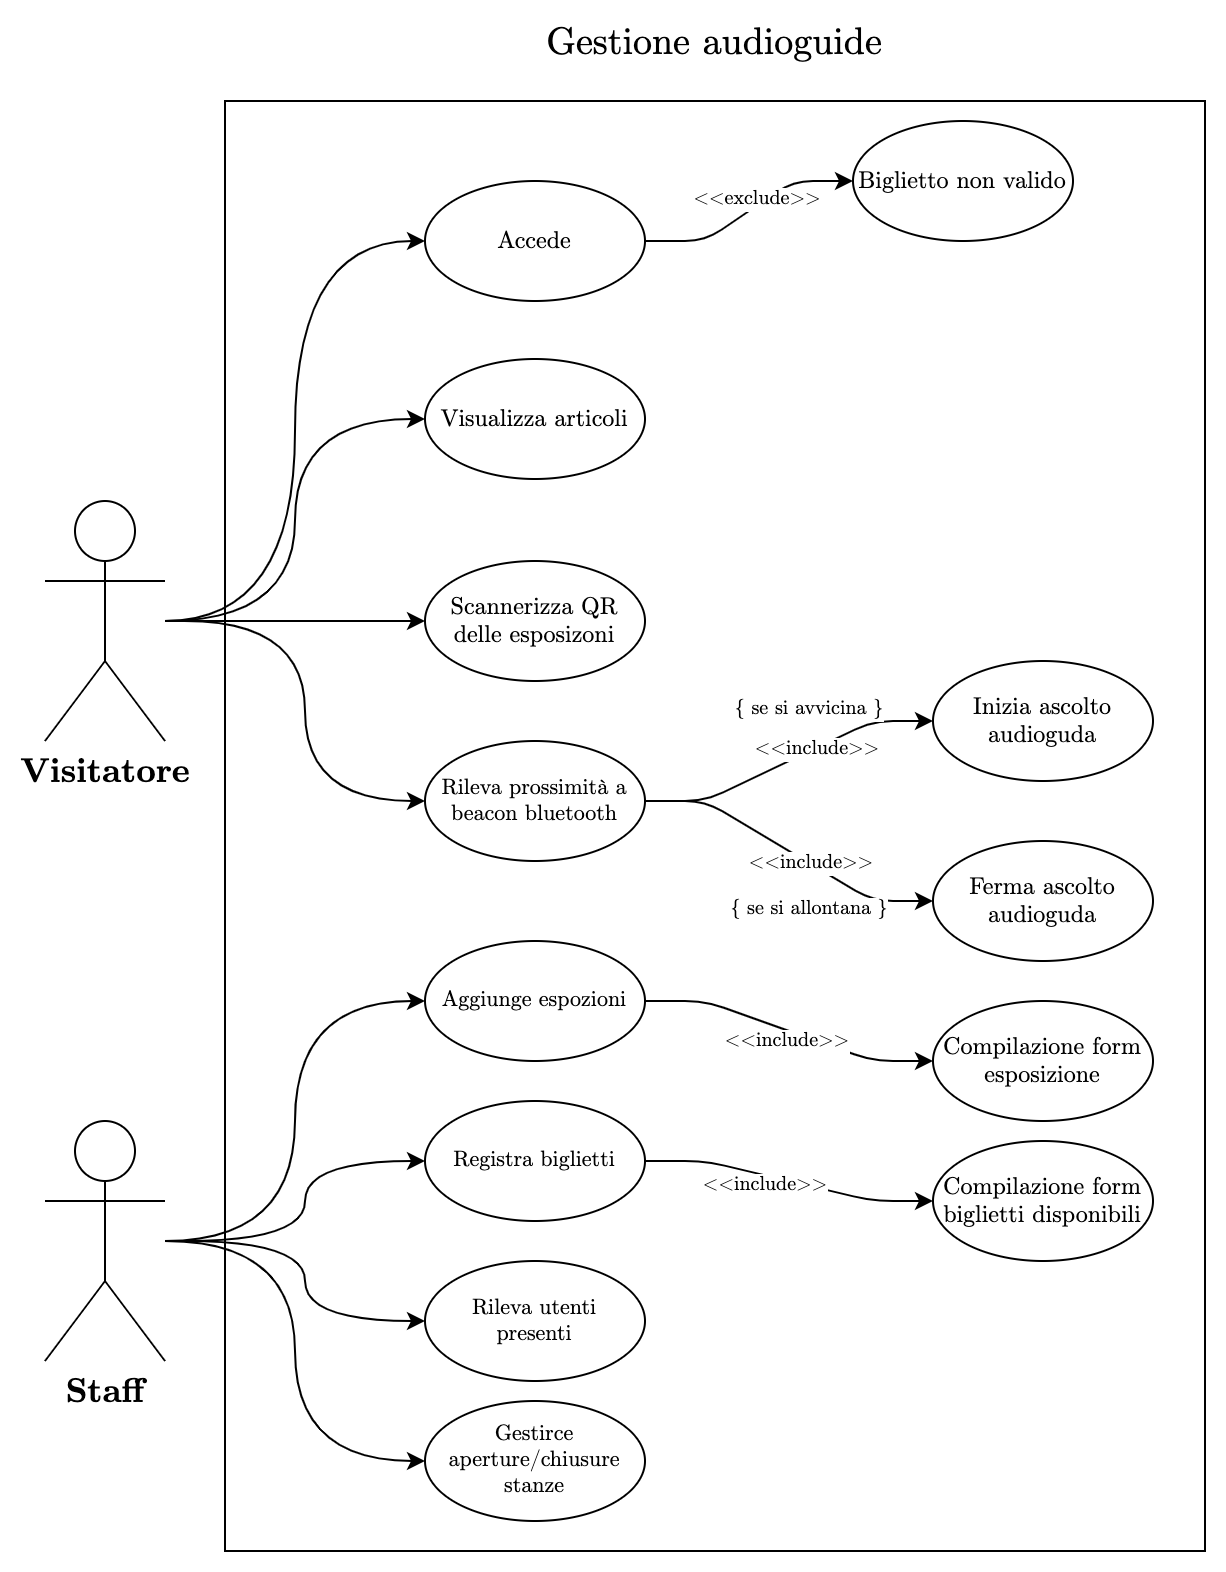
\includegraphics[width=7cm]{diagrams/usecase_diagrams.png}
        \caption{Diagramma dei casi d'uso}
        \label{fig:usecase}
    \end{figure}
\end{center}

\subsection{WBS}
\begin{center}
    \begin{figure}[htp]
        \centering
        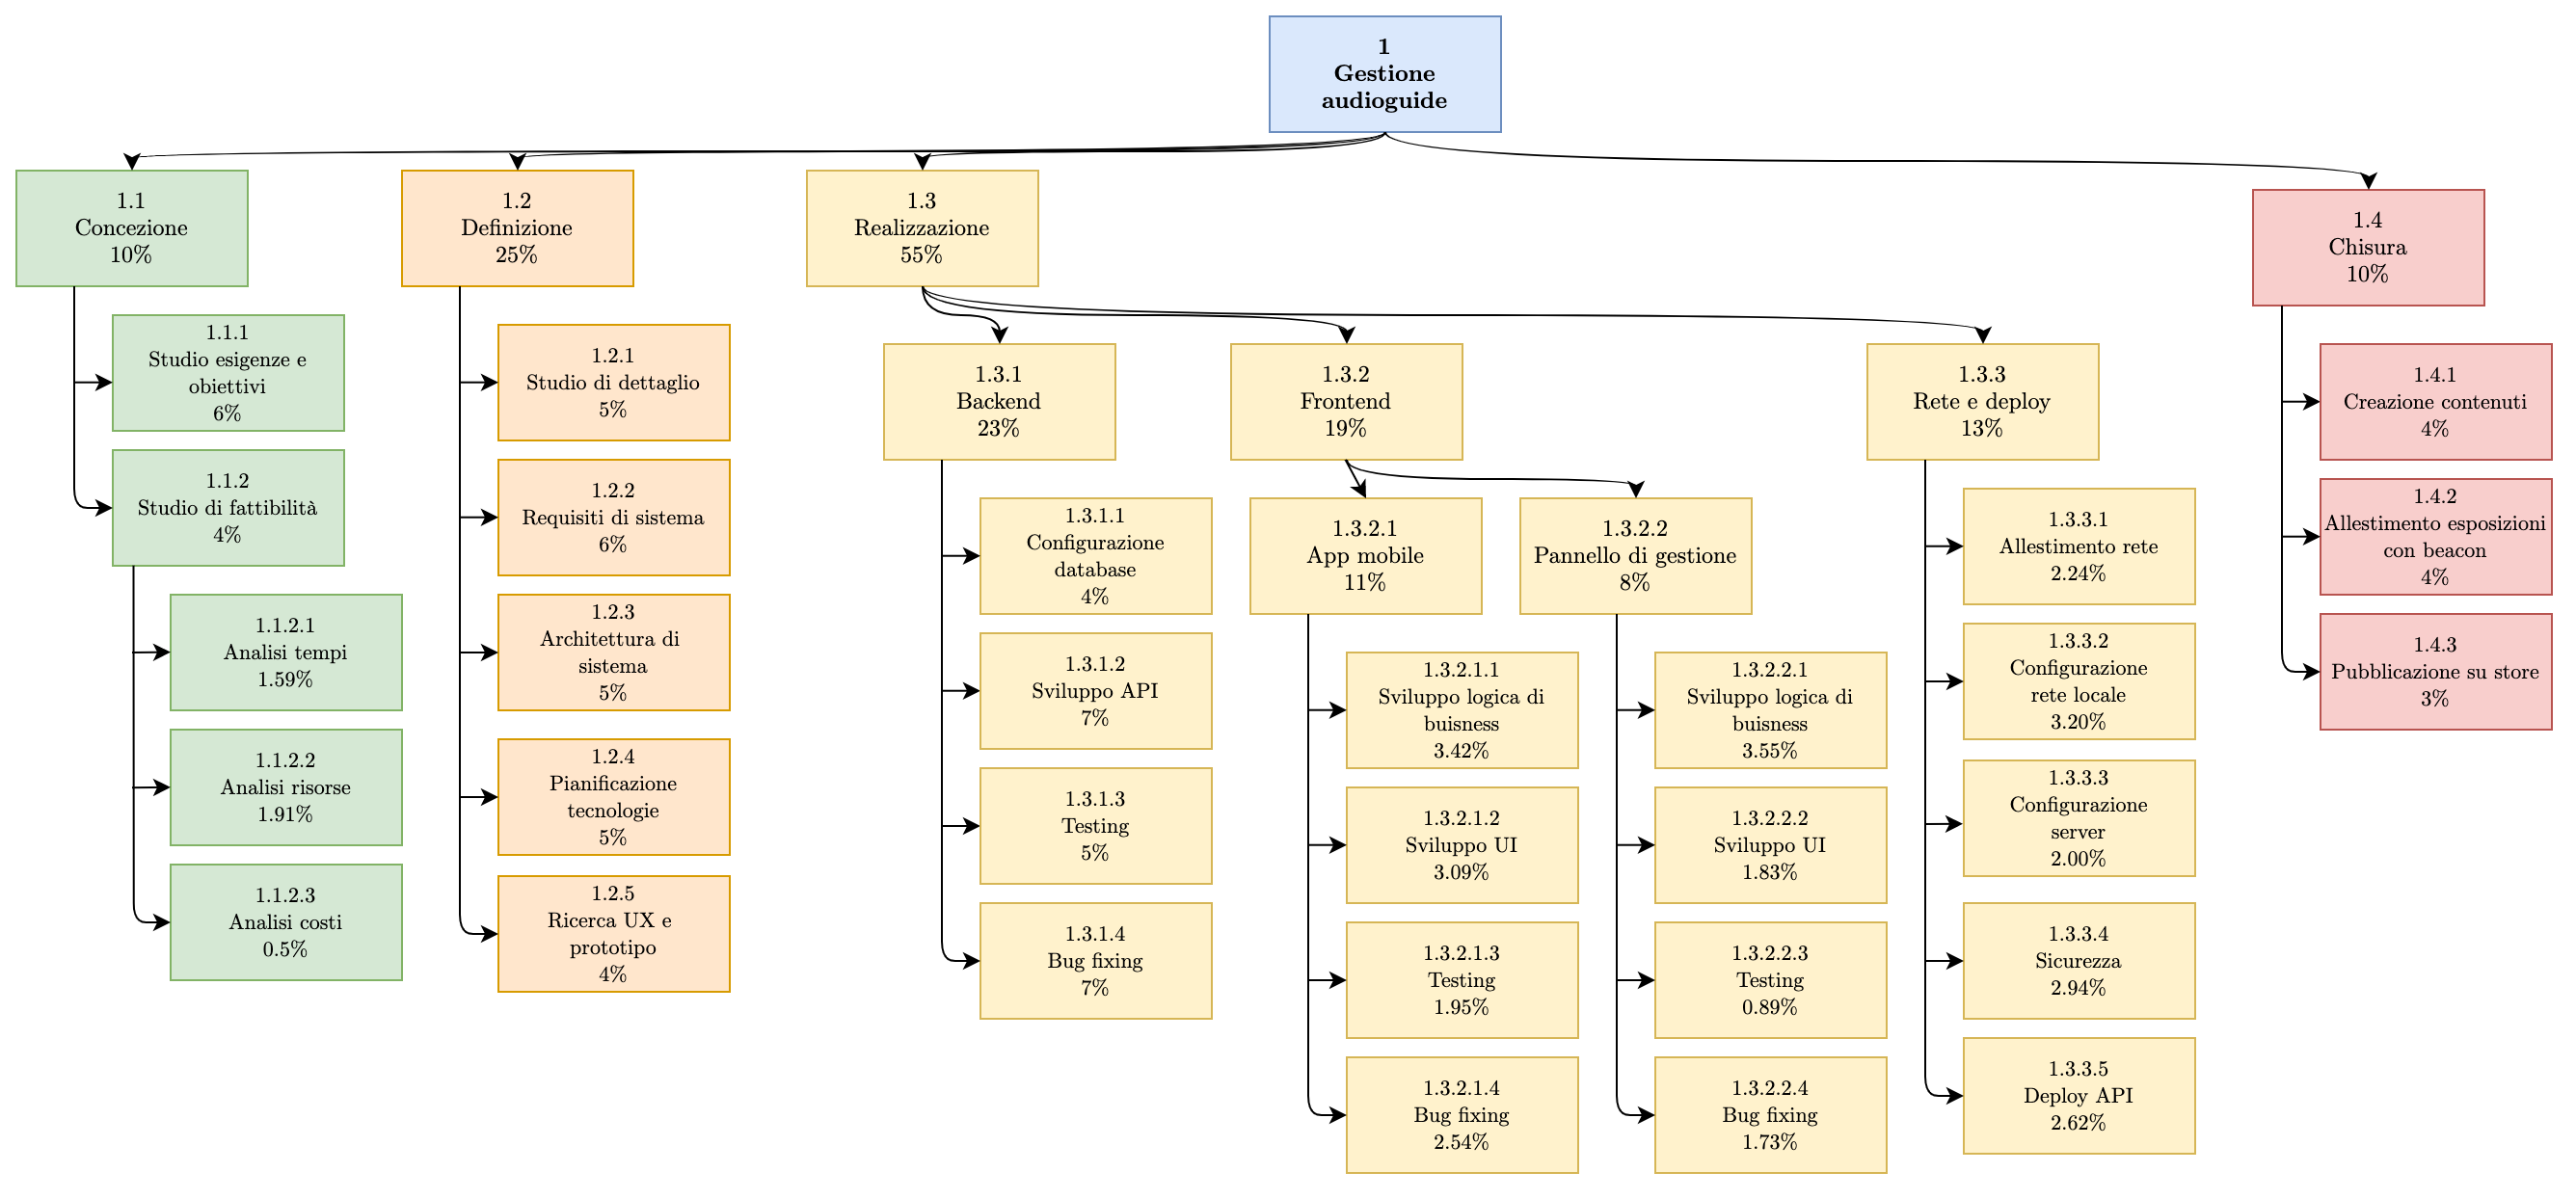
\includegraphics[width=14cm]{diagrams/elaborato_wbs_v2-wbs_V2_rev.png}
        \caption{Work Breakdown Structure}
        \label{fig:wbs}
    \end{figure}
\end{center}
\clearpage

\subfile{sections/infrastructure/infra}
\clearpage
\section{Il backend}
Il back-end, cioè la parte di ogni sito web o applicazione che gli utenti non vedono è composto da:
\begin{itemize}
    \item \textbf{server}: è il luogo in cui l'applicazione viene contenuta ed eseguita
    \item \textbf{applicazione}: l'applicazione che viene eseguita nel server, in questo caso si occupa di esporre delle API di tipo REST e di gestire il pannello di amministrazione
    \item \textbf{database}: la base dati, contiene tutti i dati necessari per l'utilizzo dell'applicazione  
\end{itemize}

\subsection{Il database}

Il database svolge una parte fondamentale di questa applicazione, per descriverlo ci sono vari metodi, qui si è scelto di trattare lo schema entità relazioni e quello logico. Come DBMS è stato usato MySQL.

\subsubsection{Schema E/R}
Lo schema E/R traduce le problematiche reali in uno  schema concettuale facilmente comprensibile, senza occuparsi di come sarà costruito il database.

\begin{center}
    \begin{figure}[htp]
        \centering
        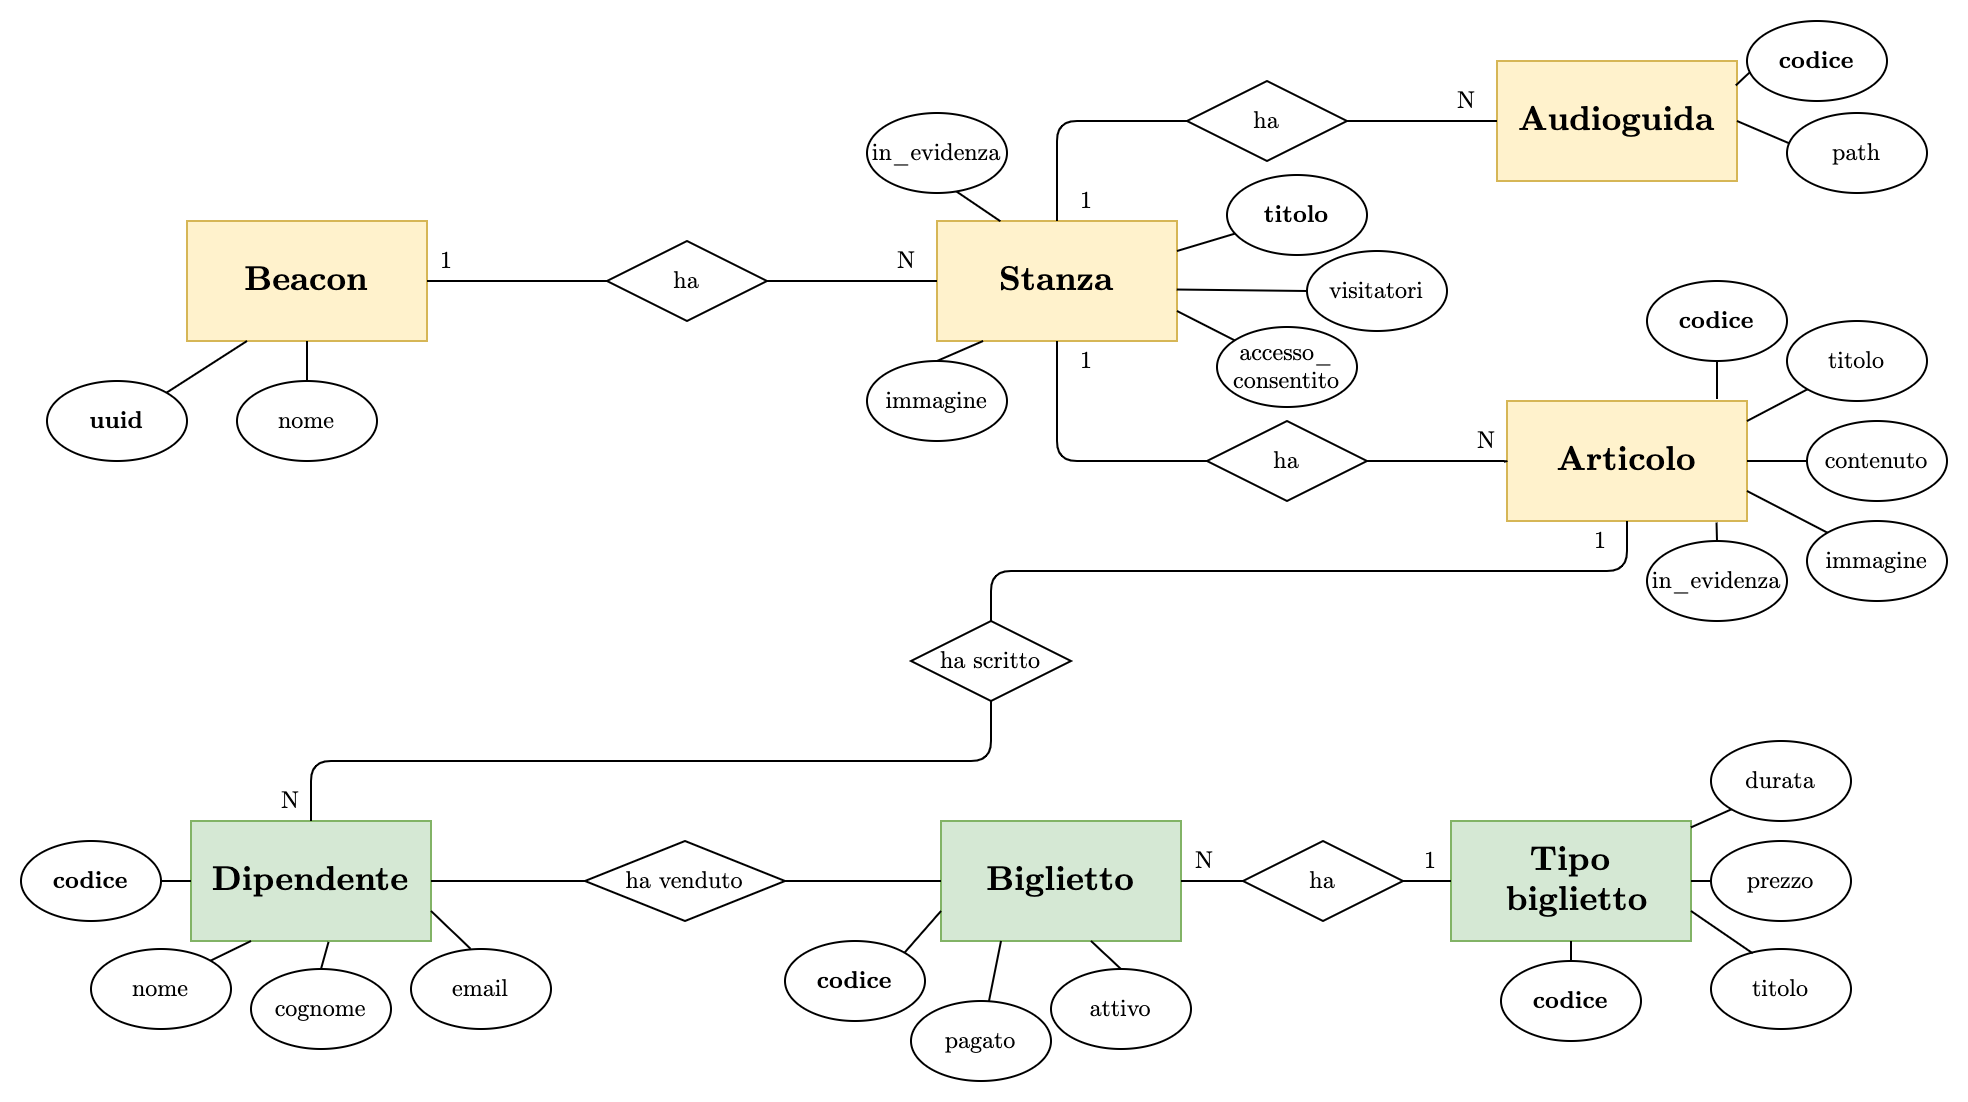
\includegraphics[width=14cm]{diagrams/er_scheme.png}
        \caption{Schema E/R}
        \label{fig:er}
    \end{figure}
\end{center}

\clearpage

\subsubsection{Schema logico}
L’obiettivo di questa fase è pervenire, a partire dallo schema concettuale, a uno schema logico che
lo rappresenti in modo fedele, “efficiente” e indipendente dal particolare DBMS adottato. Questo modello logico viene sviluppato anche per arricchire il modello concettuale visto precedentemente definendo esplicitamente le colonne di ogni entità e introducendo entità operative e transazionali.

\begin{center}
    \begin{figure}[htp]
        \centering
        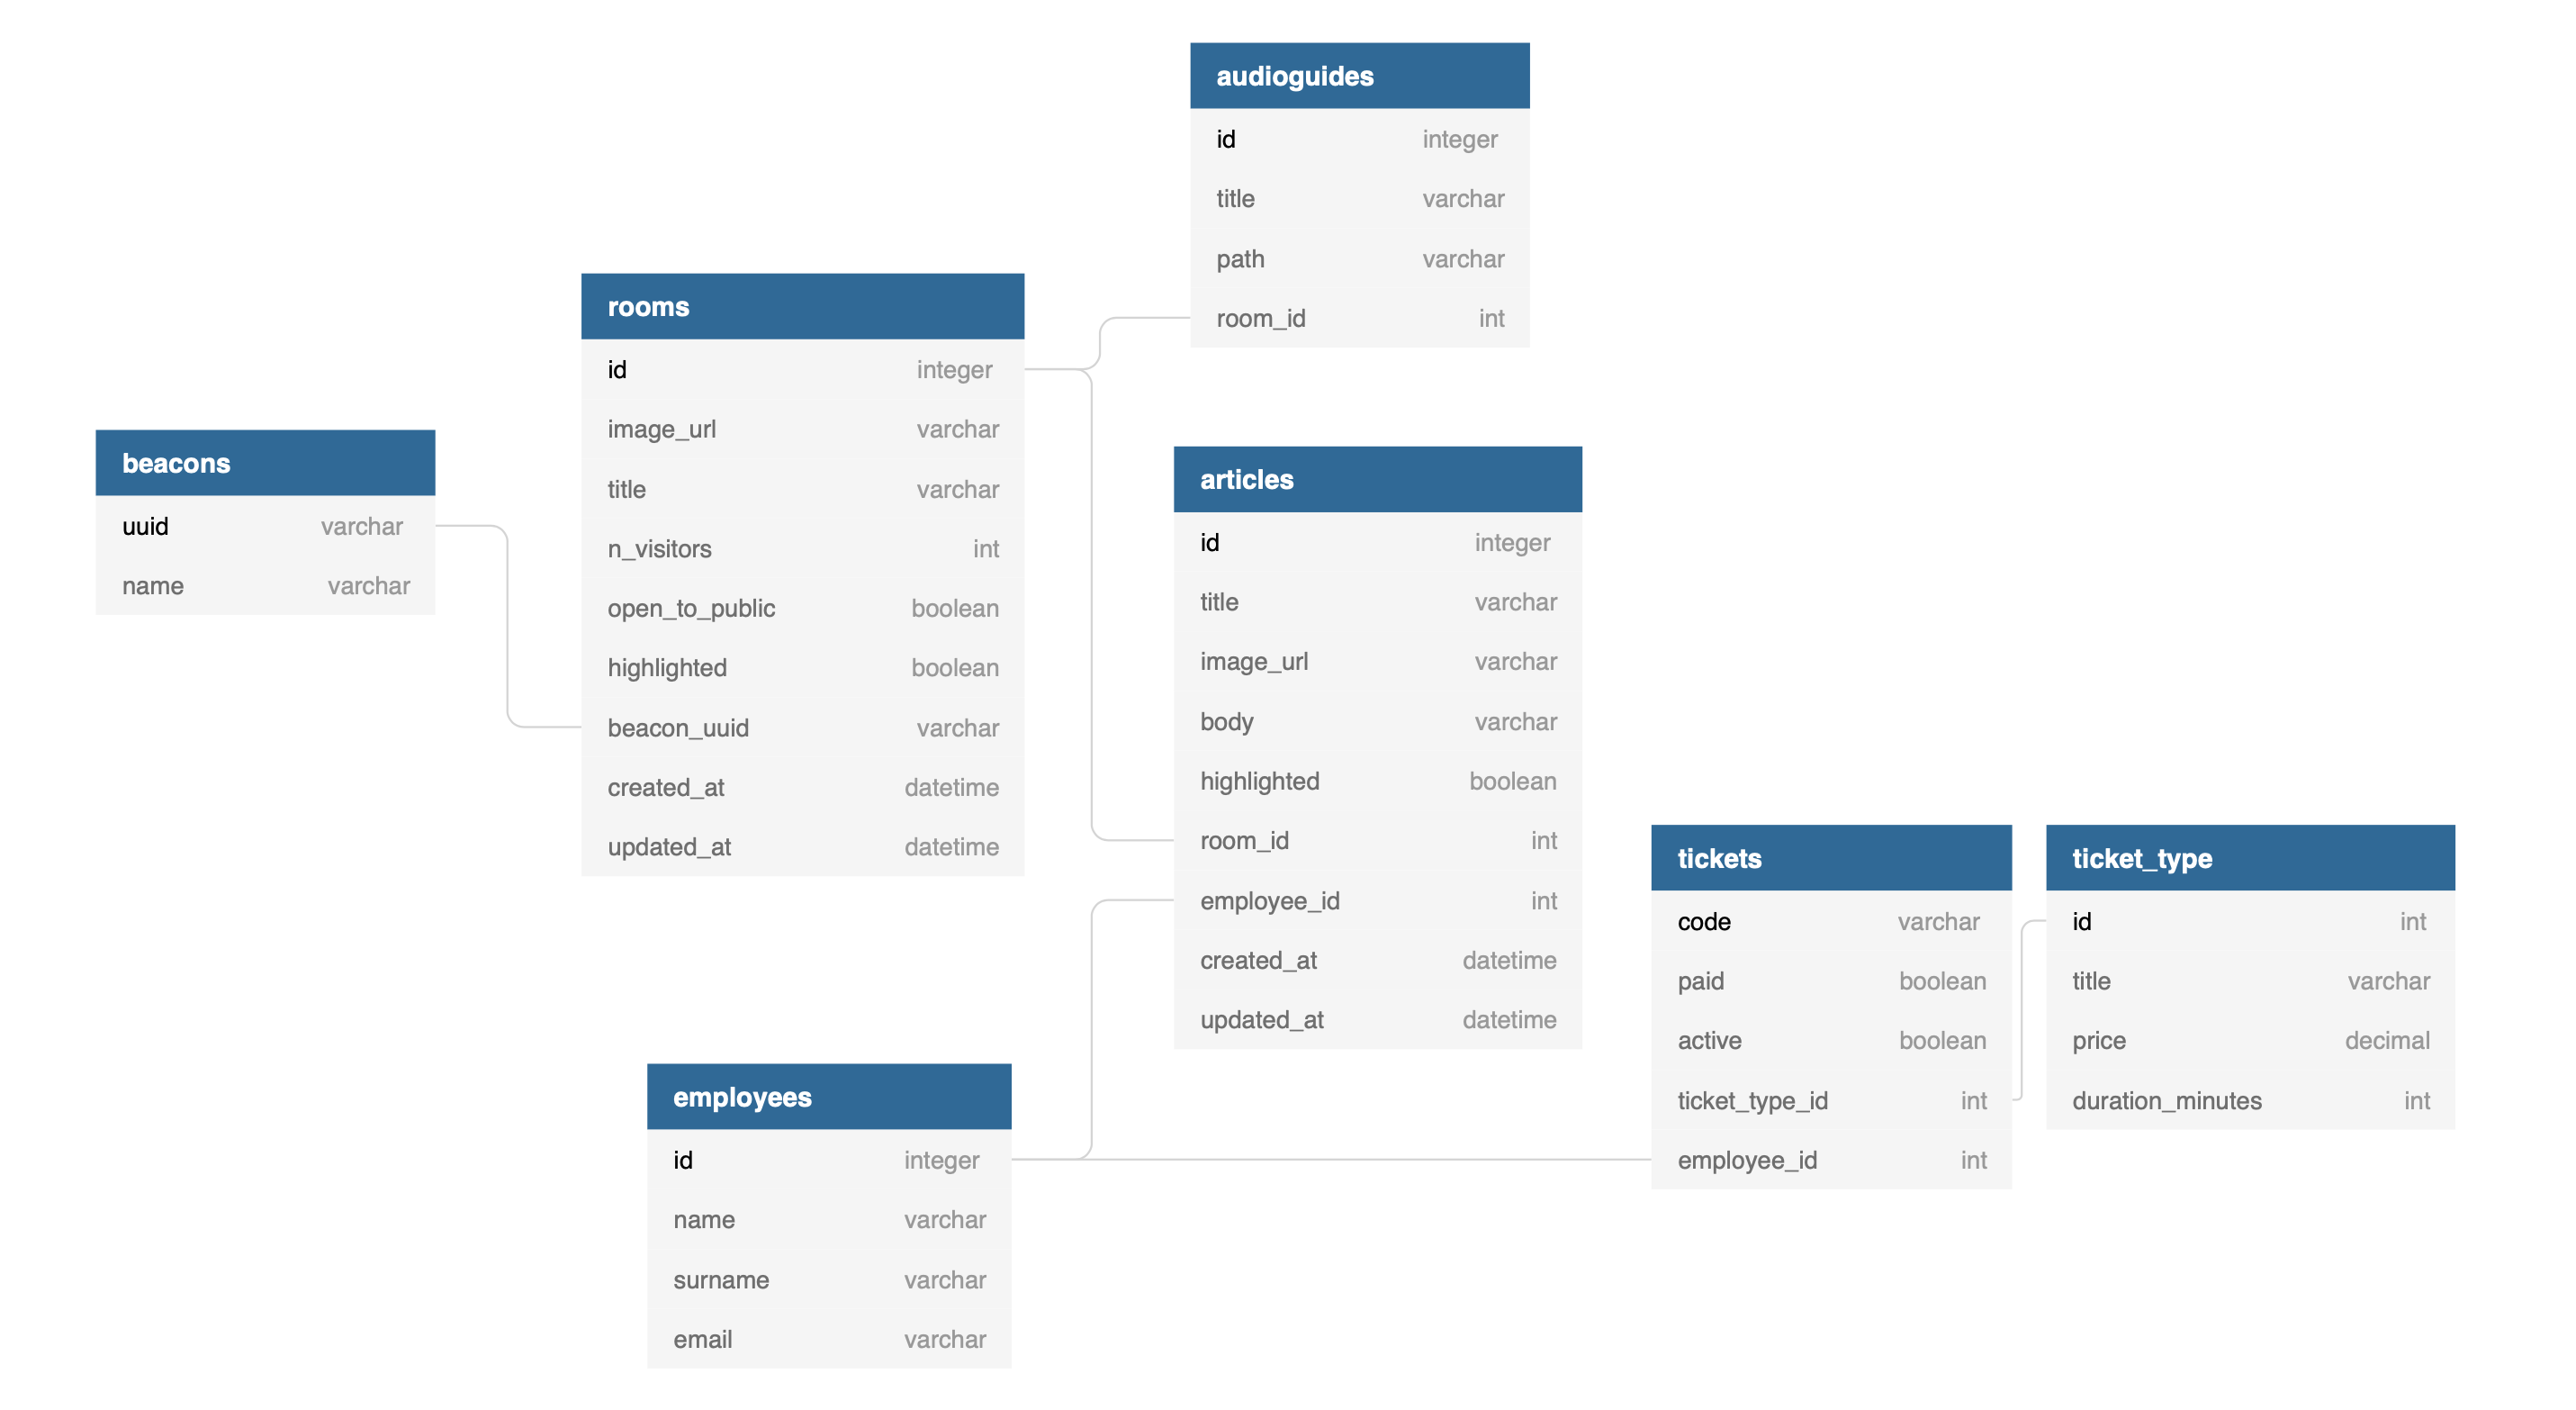
\includegraphics[width=\textwidth]{diagrams/logic_scheme.png}
        \caption{Schema logico}
        \label{fig:logic_scheme}
    \end{figure}
\end{center}

\subsubsection{API in PHP}
Le API realizzate con il framework \textbf{Lumen} offrono vari endpoint che conformano allo stile \textbf{REST} (Representational state transfer). Alcuni di questi sono:
\begin{itemize}
    \item \verb+/api/v1/rooms+: lista delle stanze
    \item \verb+/api/v1/audioguides+: lista delle audioguide
    \item \verb+/api/v1/articles+: lista degli articoli
    \item \verb+/api/v1/audioguides/{beacon_id}+: audioguide per il beacon indicato
\end{itemize}
Questi restituiscono i dati ottenuti dal database con le query in formato \textbf{JSON}, un formato adatto all'interscambio di dati fra applicazioni client/server.
\subsubsection{Query SQL}
Per ottenere i dati il server esegue delle interrogazioni al database, di cui prima è stata descritta la struttura. Di seguito vengono riportate alcune query significative; i parametri vengono indicati con le parentesi graffe, nel codice PHP sono stati ineriti tramite PDO per evitare le SQL injection.\\\\\subfile{sections/backend/queries}

\section{Il client}
\subsection{App mobile}
L'applicazione viene scaricata dai visitatori attraverso un QRCode. Avviata
e inserito il codice presente nel biglietto, l’app viene impostata per la visita alla villa. Avviene poi l'interazione con i beacon bluetooth; quando l’app rileva che l'utente sta entrando nel range del trasmettitore avvisa il sistema che il visitatore è nella stanza e manda in esecuzione il commento audio. Quando l’app non percepisce più il beacon, avvisa  che l’utente è uscito e termina la presentazione.

\subsubsection{L'architettura del codice}
L’architettura di un sistema software è la “forma” data a quel sistema da coloro che la costruiscono. Per  “forma” si intende la divisione di tale sistema in componenti, nella disposizione di essi e nei modi in cui tali componenti comunicano tra loro. Lo scopo è  quello di facilitare lo sviluppo, la distribuzione, il funzionamento e la manutenzione del sistema software in esso contenuto.\cite{architettura_codice}
Come architettura è stato deciso di usare la \textbf{clean architecture}, il cui scopo principale è quello di permettere al business di adattarsi ai cambiamenti della tecnologia e delle interfacce cambiando il meno codice possibile. Aiuta a rimuovere quello stretto accoppiamento tra la logica di business e il livello di presentazione.\cite{architettura_introduction}\clearpage Questo tipo di architettura ha tre livelli principali:
\begin{itemize}
    \item \textbf{Presentazione}: contiene tutta la UI, si tratta principalmente di codice Flutter. 
    \item \textbf{Dominio:} è dove si definiscono le entità e i casi d'uso. Non vi sono classi concrete, solo interfacce (classi astratte). Tutte le implementazioni sono nel livello più sotto, il \emph{data}. 
    \item \textbf{Data}: questo livello è responsabile di tutte le implementazioni dei casi d'uso e delle interfacce. Solitamente contiene classi per l'accesso ai dati del database o di una sorgente remota.
\end{itemize}

\begin{center}
\begin{figure}[htp]
    \centering
    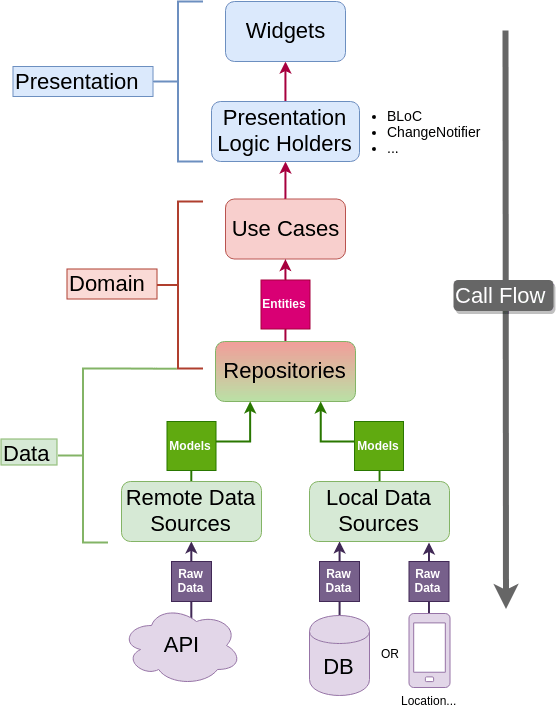
\includegraphics[height=10cm]{diagrams/clean_architecture.png}
    \caption{Lo schema della clean architecture}
    \label{fig:clean_architecture}
\end{figure}
\end{center}

\subsubsection{La gestione dello stato}
Un’applicazione non è mai del tutto statica e richiede in quasi tutti i casi di:
\begin{itemize}
	\item tracciare i cambiamenti
	\item dare l’opportunità all’utente di poter interagire con la UI
	\item aggiornare la UI dinamicamente in caso di cambiamenti nelle informazioni mostrate.
\end{itemize}
Per gestire tutti questi aspetti in Flutter è possibile utilizzare una soluzione più elegante rispetto ai widget \emph{stateful}, il \textbf{BloC Pattern}. Questo pattern, che è implementato su Flutter con la libreria \emph{flutter\_bloc} permette di gestire il flow dell'applicazione tramite una stream di eventi.\clearpage
Di seguito è riportato il diagramma degli stati, una rappresentazione che descrive il comportamento dei sistemi analizzando gli stati, le transizioni e le azioni.

\begin{center}
    \begin{figure}[htp]
        \centering
        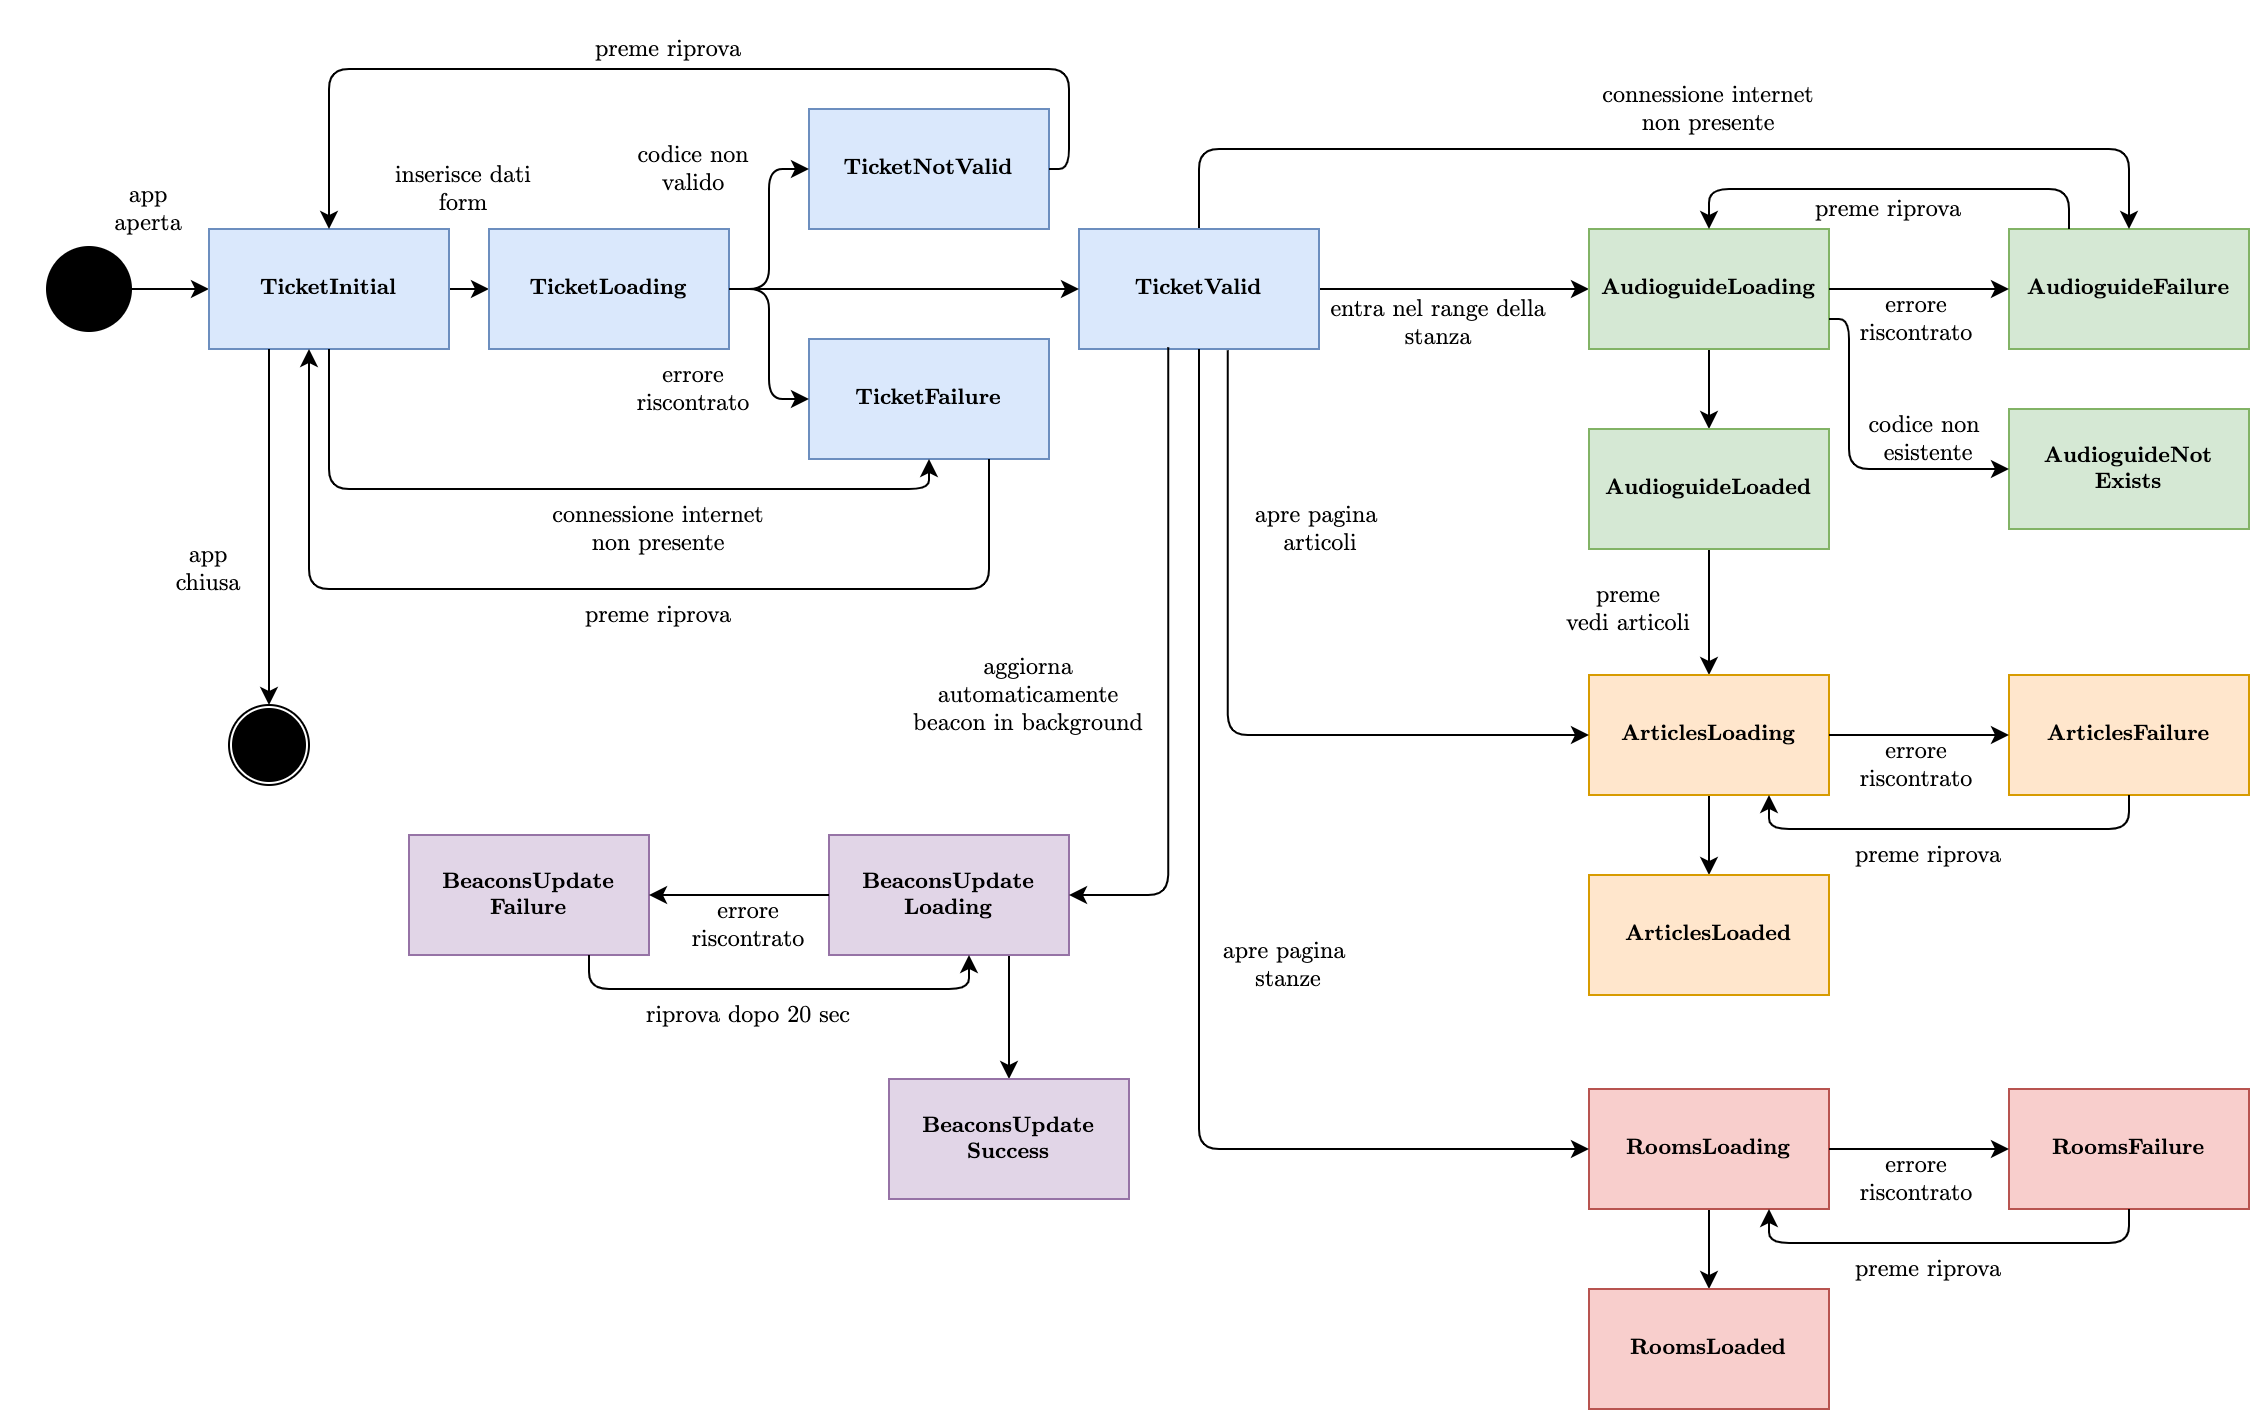
\includegraphics[height=11cm]{diagrams/state_diagrams.png}
        \caption{Il diagramma degli stati}
        \label{fig:state_diagrans}
    \end{figure}
\end{center}
    

\subsection{Pannello di amministrazione web}
Il pannello di amministrazione permette di:
\begin{itemize}
    \item gestire la vendita dei biglietti
    \item osservare il conteggio effettivo dei visitatori
    \item chiudere o aprire l’accesso alle stanze
\end{itemize}
L'accesso è limitato, può essere visualizzato soltanto dallo staff. Per realizzarlo è stato usato il framework PHP \textbf{Laravel}. L'applicativo accede allo stesso database delle API Rest ma è totalmente separato in termini di codice. 

\subfile{sections/frontend/admin_panel.tex}

\subfile{sections/security/security.tex}

\section{Considerazioni finali}
\subsection{Esperienza PCTO}
I moduli curriculari PCTO svolti durante i tre anni sono stati estremamente utili per la realizzazione di questo progetto; le competenze di \textbf{autoapprendimento} mi hanno aiutato a imparare ed utilizzare nuove tecnologie che non avevo mai usato, come ad esempio il framework \emph{Laravel}. Le competenze di \textbf{analisi di sistemi} mi hanno permesso di analizzare e risolvere con metodologia i vari problemi incontrati durante la realizzazione; infine l'attività svolta in quarta -\emph{Sviluppo App per Web e mobile}- ha arricchito notevolmente le mie competenze per quanto riguarda la creazione di un applicativo complesso e distribuito su più piattaforme.

\subsection{Risultati raggiunti e futuri miglioramenti}
Alla conclusione di questo elaborato, il cui obiettivo era quello di sviluppare una applicazione full-stack per semplificare notevolmente l'utilizzo delle audioguide, sia da parte dell'operatore che dell'utente finale, è possibile affermare che, sulla base dei test effettuati sulle funzionalità implementate, l'applicazione rappresenta un buon punto di partenza per lo sviluppo del prodotto finale. Alcune future funzionalità potrebbero comprendere:
\begin{itemize}
    \item aggiunta di un quiz per far interagire gli utenti con l'esposizione
    \item aggiunta di video o altri contenuti multimediali per comprendere meglio la spiegazione
    \item possibilità di maggiore personalizzazione dell'applicazione dal pannello di gestione
\end{itemize} 


\subsection{Conclusioni}


Il mobile computing è ogni giorno più presente nella nostra routine quotidiana. Questo può essere spiegato dalla grande evoluzione che si è verificata in questo settore nel corso dell'ultimo decennio e che ha causato l'emergere di una varietà di nuovi dispositivi mobili e sistemi operativi, sempre più sofisticati e potenti.  Attraverso l'internet of things è possibile collegare a questi dispositivi una miriade di gadget e scambiare informazioni, creando delle integrazioni che semplificano sempre di più la nostra vita quotidiana e migliorano le esperienze d'uso.

\printbibliography

\end{document}

